% !TEX root =  ../main.tex
\section{SplitAmong}

\subsection{Definition}

\subsubsection{Signature} \cstr{splitAmong(vs : set<set<VM>>, ns : set<set<server>>)}

\begin{itemize}
\item \cstr{vs} : a non-empty set of set of VMs for a meaningful constraint. VMs not in the \st{Running} state are ignored. Sets inside \cstr{vs} must be disjoint.
\item \cstr{ns} : a set of set of servers that is composed of more sets than \cstr{vs} or the constraint is sure of not being satisfiable.
Sets composing \cstr{ns} must be disjoint. Servers not in the \st{Online} state are ignored.
\end{itemize}

The \cstr{splitAmong} constraint forces the sets of VMs inside \cstr{vs}
to be hosted on distinct set of servers in \cstr{ns}. VMs inside a same set may still be collocated.

\classification{splitAmong}{application administrator}{VM placement}{VM-to-VM placement,Partitioning,Fault tolerance}

\subsubsection{Usage}

The \cstr{splitAmong} constraint deserves isolation requirements. One solution to ensure disaster recovery for an application is to replicate it. When the master application fail, the replica is activated transparently to neglect the failure effect. In practice, the replication is a mechanism provided at the hypervisor level~\cite{remus,vmwareFT}. The replicas are then placed to a distant server to make the application survive
to a datacenter failure. One application administrator may obtain this fault tolerance using one \cstr{splitAmong} constraint. The sets of VMs given as parameters are the master then the slave VMs while the
set of servers are the servers composing each datacenter.

\subsubsection{Example}

Figure~\ref{fig: splitAmong} depicts a sample reconfiguration between a source and a destination configuration. In this example, the following \cstr{splitAmong} constraints were considered:

\begin{reconfiguration}
\centering
\begin{minipage}[b]{0.40\textwidth}
\begin{lstlisting}
N1: VM1 VM2
N2: VM3
N3: VM4 VM5
N4: VM6
N5: VM7 VM8
\end{lstlisting}
\end{minipage}
\begin{minipage}[b]{2cm}
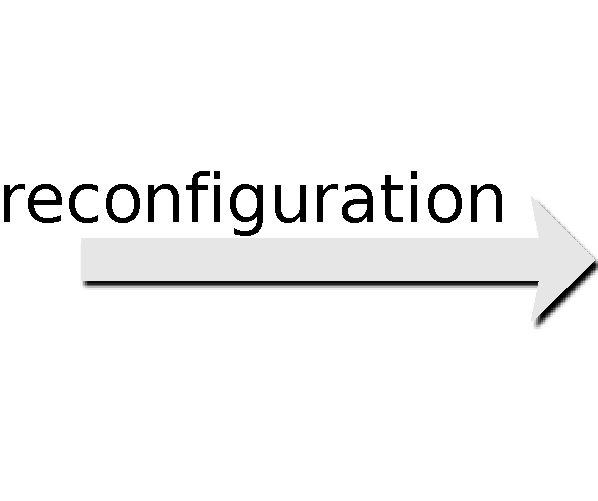
\includegraphics[width=2cm]{img/arrow_reconfiguration}
\end{minipage}
\begin{minipage}[b]{0.40\textwidth}
\begin{lstlisting}
N1: VM1
N2: VM3
N3: VM2 VM4 VM5
N4: VM7 VM6
N5: (VM8)
\end{lstlisting}
\end{minipage}
\caption{A reconfiguration motivated by \cstr{splitAmong} constraints.}\label{fig: splitAmong}
\end{reconfiguration}


\begin{itemize}

\item \cstr{splitAmong(\{\{VM1,VM3\},\{VM2,VM4\}\},\{\{N1,N2\},\{N3,N4\}\})}. This constraint was not satisfied in the source configuration as \cstr{VM2} and \cstr{VM1} were both running inside the set of servers \cstr{\{N1,N2\}} despite they belong to different sets of VMs. In addition, the set of VMs \cstr{\{VM2,VM4\}} was spread among the two set of servers while it should be running on only one. These violations were fixed by relocating \cstr{VM2} to \cstr{N4} to let the first set of VMs running on the first set of servers and the second set of VMs running on the second set of servers.

\item \cstr{splitAmong(\{\{VM1,VM3\},\{VM5,VM6,VM7, VM8\}\},\{\{N1,N2\},\{N3,N4\}\})}. This constraint was not satisfied in the source configuration as \cstr{VM7} and \cstr{VM8} were running on \cstr{N5}, that does not belong to any of the allowed sets.  This violation was fixed by relocating \cstr{VM7} to \cstr{N4} and by suspending \cstr{VM8} which is now ignored by the constraint.

\item \cstr{splitAmong(\{\{VM1,VM2,VM3\},\{VM7,VM8\}\},\{\{N1,N2,N3\},\{N4,N5\}\})}.This constraint was satisfied in the source configuration as the sets of VMs share do not share a group of servers. The constraint is still satisfied in the destination configuration despite the relocation of \cstr{VM2} and \cstr{VM7} to \cstr{N3} and \cstr{N4} respectively which let them running inside their dedicated group of servers.

\end{itemize}

%Availability: FT VMWare and EC2
\subsection{See also}

\subsubsection{Related Constraints}
\begin{itemize}
\item \cstrref{split}: This constraint disallows two set of VMs to share servers.
\item \cstrref{spread}, \cstrref{lazySpread}: These constraints disallow the colocation between VMs rather than groups of VMs.
\item \cstrref{fence}: \cstr{splitAmong} is equivalent to a \cstr{fence} constraint when only one set of VMs and one set of servers are given as arguments.

\end{itemize}

\printListOfInheritance{splitAmong}